\section{Results}

% Detallad en este apartado los resultados obtenidos utilizando la metodología descrita en el apartado anterior.

\subsection{MSI-1's RRM1-orig docking model}

The first docking simulation performed with \texttt{LightDock} corresponded to the RRM1-orig RNA-motif complex. The simulation yielded several models out of which 10 were visualized, as shown in \textbf{Figure \ref{fig:allRRMorig}}:

\begin{figure}[htbp!]
    \centering
    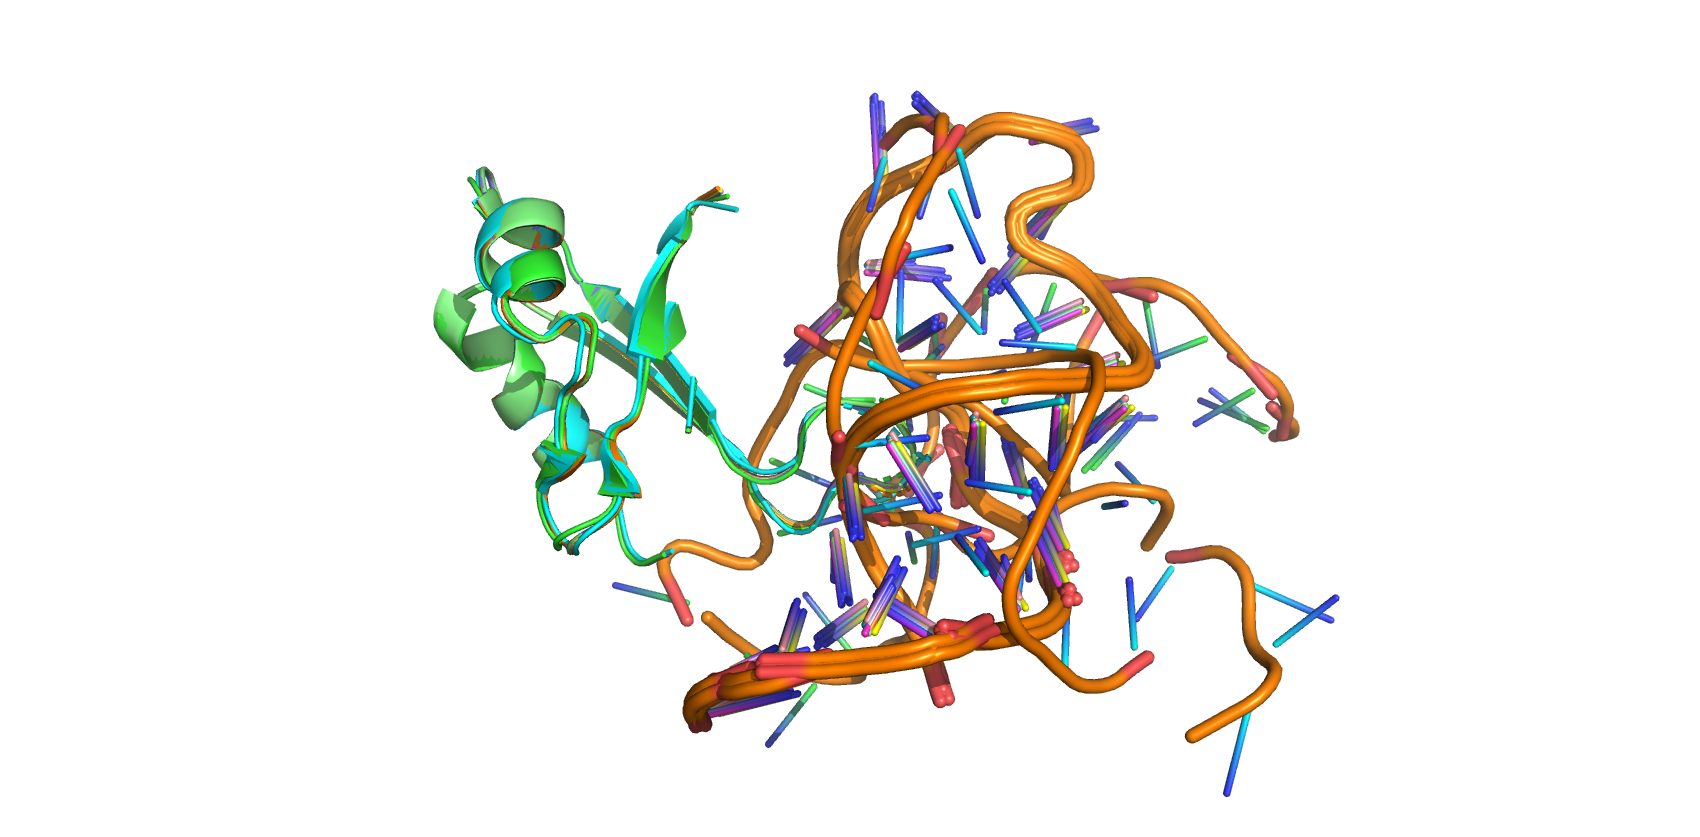
\includegraphics[width=0.82\linewidth]{assets/RMM1_orig_ALL.png}
    \caption[Top 10 scoring models for RRM1-orig RNA-motif complex.]{Top 10 scoring models for RRM1-orig RNA-motif complex. Visualized through \href{https://pymol.org/2/}{\texttt{Pymol}}.}
    \label{fig:allRRMorig}
\end{figure}

It is observed that there is no consensus among the top 10 scoring models, as it seems that the RNA-motifs adopts different conformations. To be more precise, in \textbf{Figure \ref{fig:allRRMorig}} there are 3 different RNA conformations. Their separate conformations are shown in \textbf{Figure \ref{fig:RRMorigSep}}:

\begin{figure}[htbp!]
\minipage{0.32\textwidth}
    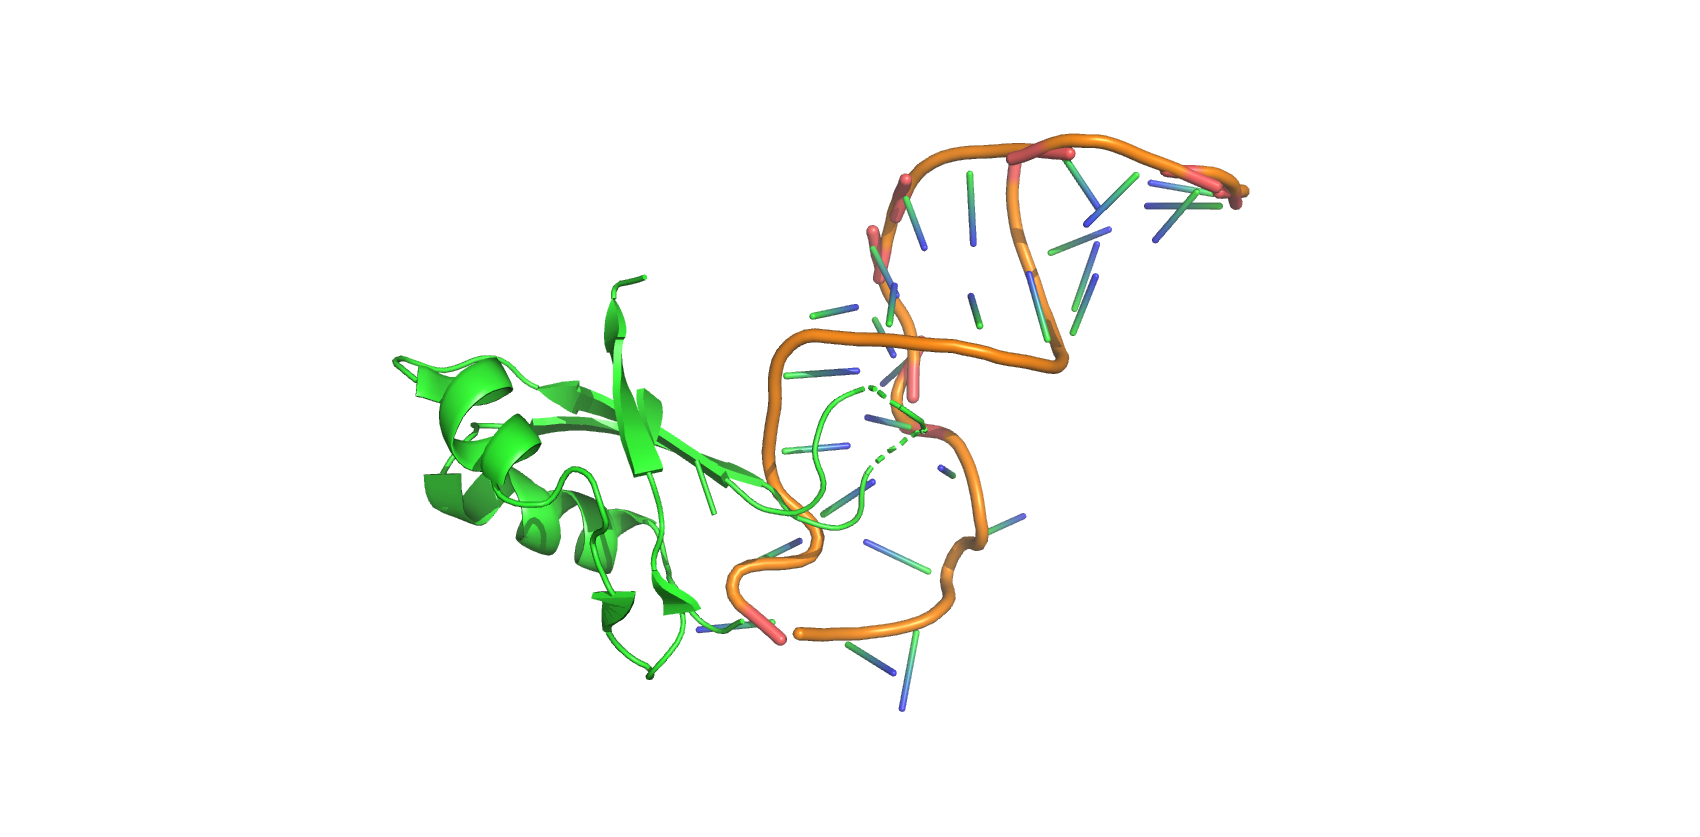
\includegraphics[trim={6.5cm 0 6.5cm 0},clip,width=\linewidth]{assets/RMM1_orig_top0.png}
\endminipage\hfill
\minipage{0.32\textwidth}
    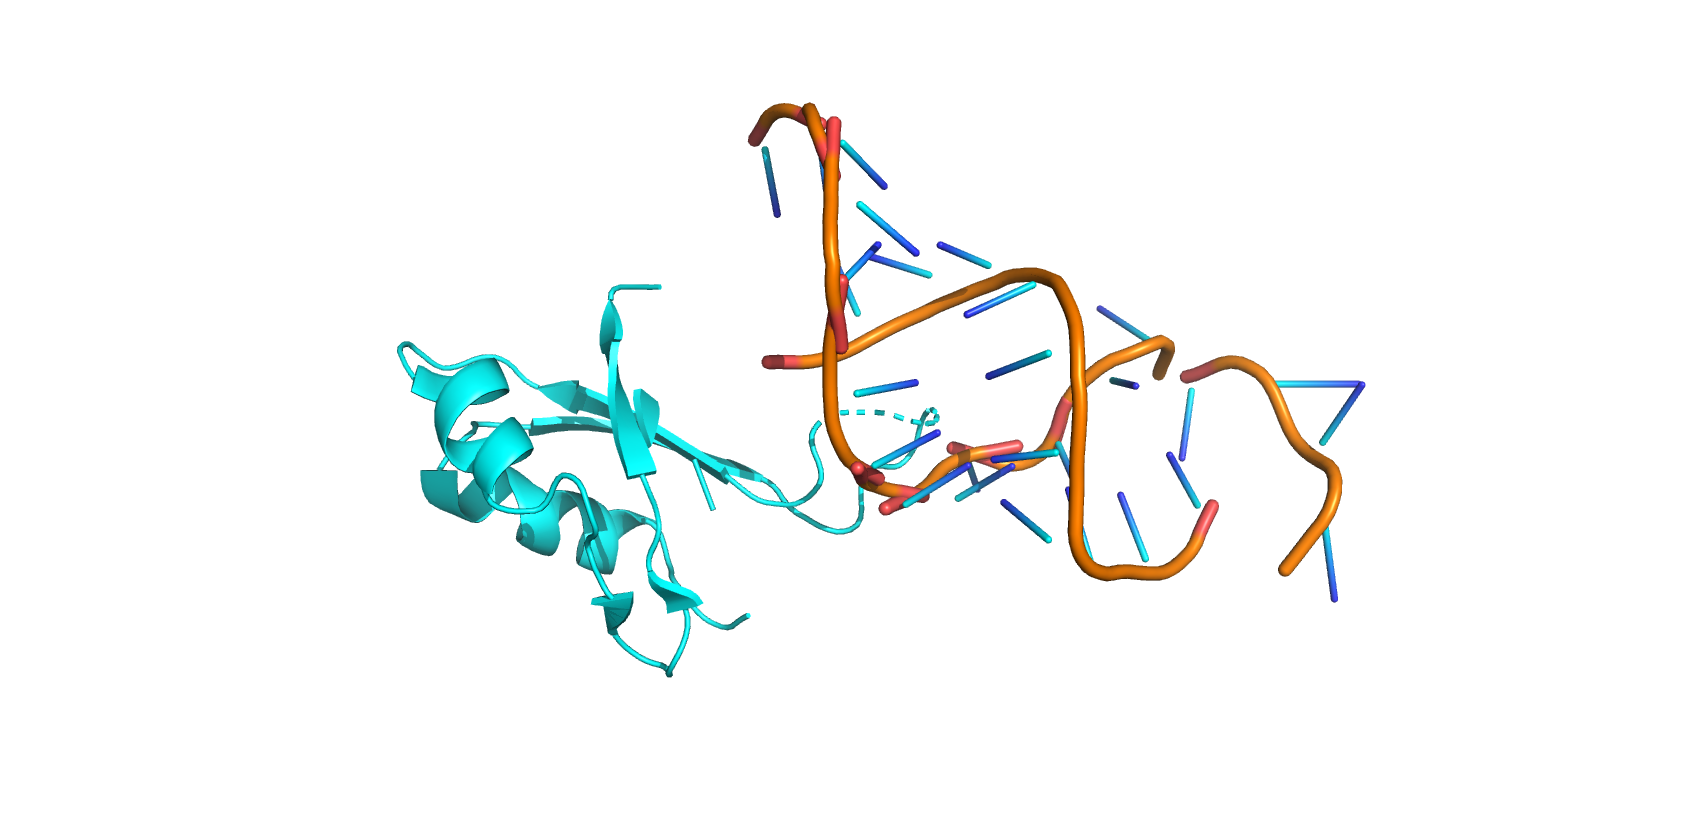
\includegraphics[trim={6.5cm 0 5.5cm 0},clip,width=\linewidth]{assets/RMM1_orig_top1.png}
\endminipage\hfill
\minipage{0.32\textwidth}
    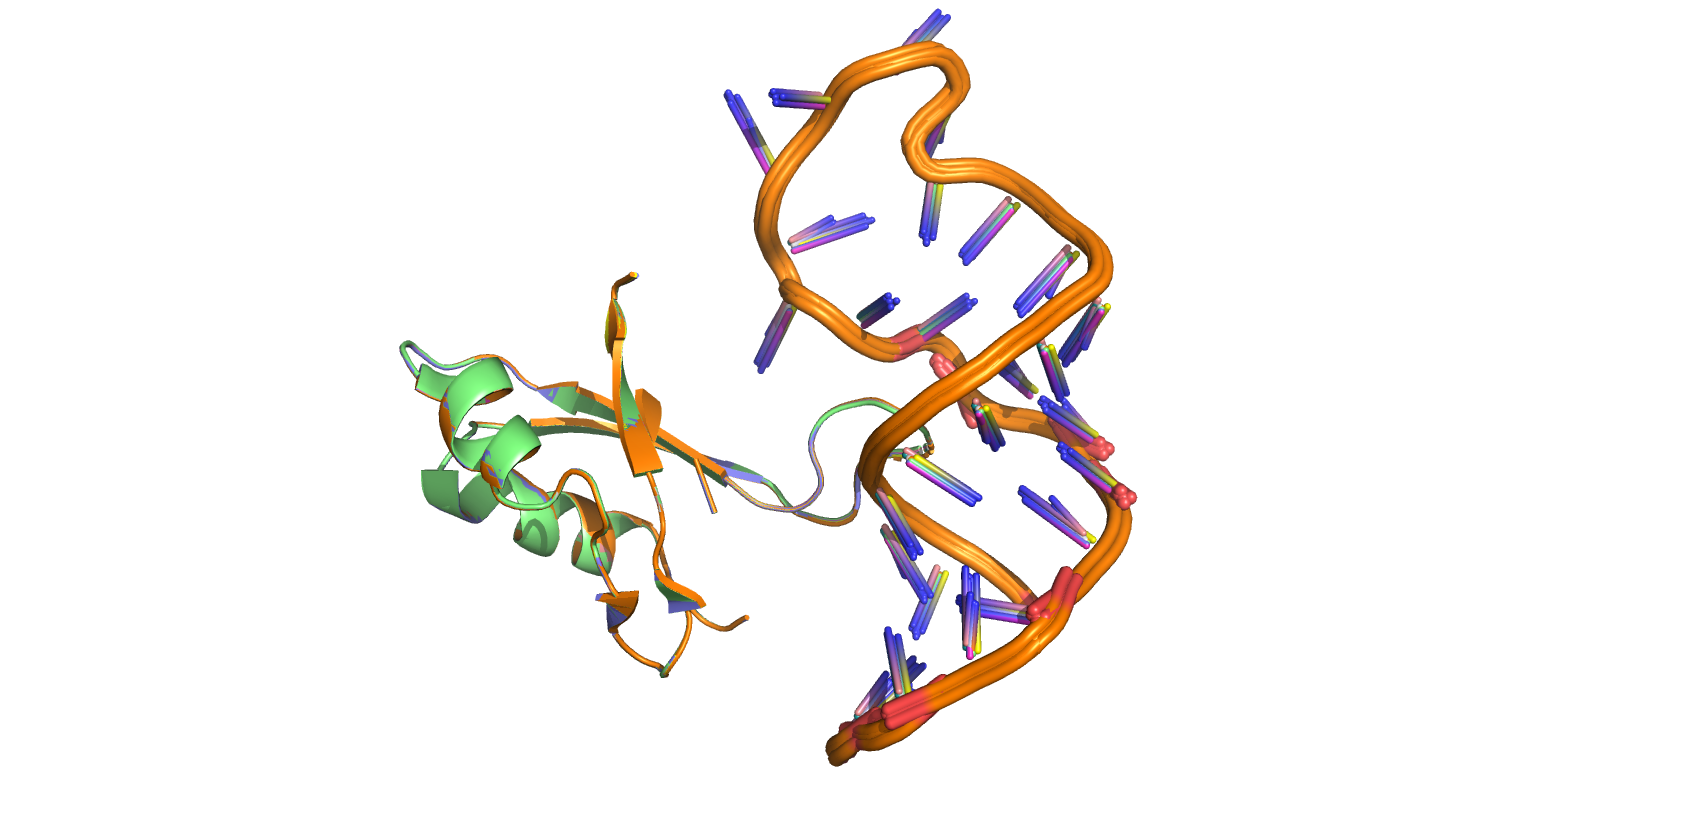
\includegraphics[trim={6.5cm 0 7cm 0},clip,width=\linewidth]{assets/RMM1_orig_2to8.png}
\endminipage
\caption[Top 10 scoring models for RRM1-orig RNA-motif complex grouped by RNA conformations.]{Top 10 scoring models for RRM1-orig RNA-motif complex grouped by RNA conformations. From left to right: best scoring model, second best scoring model and top 3 to 10 best scoring models. Visualized through \href{https://pymol.org/2/}{\texttt{Pymol}}.}
\label{fig:RRMorigSep}
\end{figure}

These models have all in common that MSI1's RRM1 interacts with the RNA motif through the \texttt{DPLTKRS}\footnote{Aspartic acid - Proline - Leucine - Threonine - Lysine - Arginine - Serine loop present in RRM1} loop by inserting itself into a groove present in the secondary structure of the RNA. Clingman and colleagues \cite{clingman_2014} observed a similar interaction with their unstructured RNA. The interactions presented in \textbf{Figure \ref{fig:RRMorigSep}} have mantained the RNA self-folding almost intact, which may not occur in reality, as proteins have natural capabilities of disrupting nucleic acid base pairing hydrogen bonds (see for example the Helicase).\\

Thus, it is natural to reason that the interaction ocurring in nature must be an intermediate structure between Clingman's usntructured RNA and the structured RNA shown in \textbf{Figure \ref{fig:RRMorigSep}}.

\subsection{MSI-1's RRM1-orig (unstructured) docking model}

To account for the scenario in which the RNA is unstructured (i.e. lacking the natural secondary structure), another docking simulation was executed, which yielded the models shown in \textbf{Figure \ref{fig:linearOrigRRM1}}:

\begin{figure}[htbp!]
    \centering
    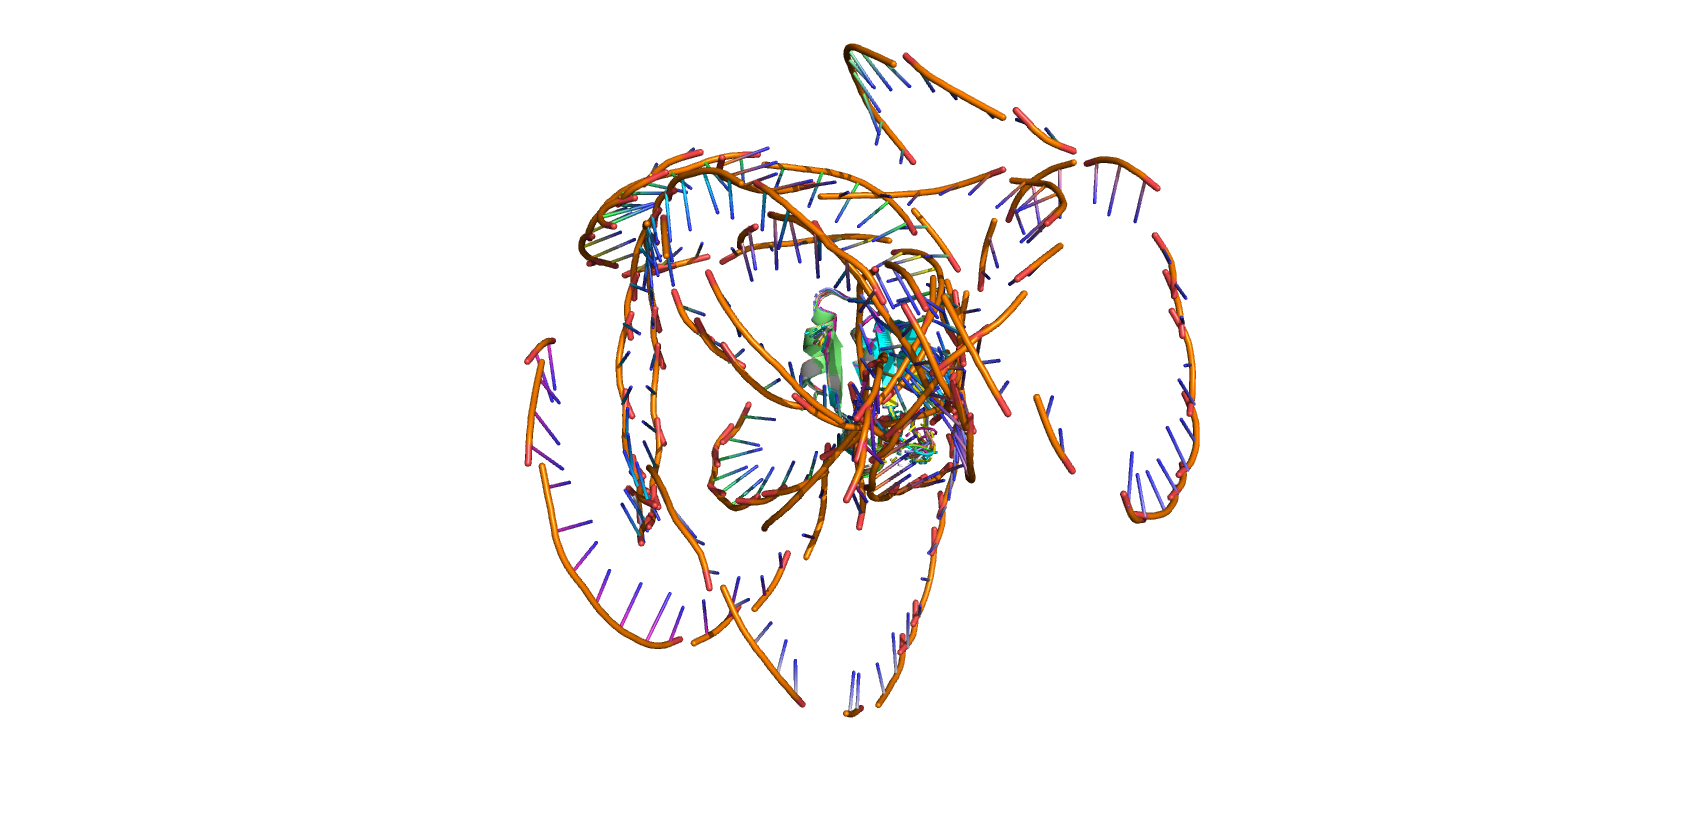
\includegraphics[width=0.82\linewidth]{assets/RMM1_linearOrig.png}
    \caption[Top 10 scoring models for RRM1-orig unstructured RNA-motif complex.]{Top 10 scoring models for RRM1-orig unstructured RNA-motif complex. Visualized through \href{https://pymol.org/2/}{\texttt{Pymol}}.}
    \label{fig:linearOrigRRM1}
\end{figure}

There is no consensus among structures. In fact, it seems that long stretches of unstructured RNA do not perform well in docking experiments, as due to the aggressiveness of the docking models, the RNA strand breaks down in multiple regions (more than their structured counterparts) and interactions seem spurious all around the protein surface.\\

\subsection{MSI-1's RRM1-mutant RNA docking models}

The simulation with each of the mutants yielded the models shown in \textbf{Figure \ref{fig:RRMmuts}}:

\begin{figure}[htbp!]
    \minipage{0.32\textwidth}
        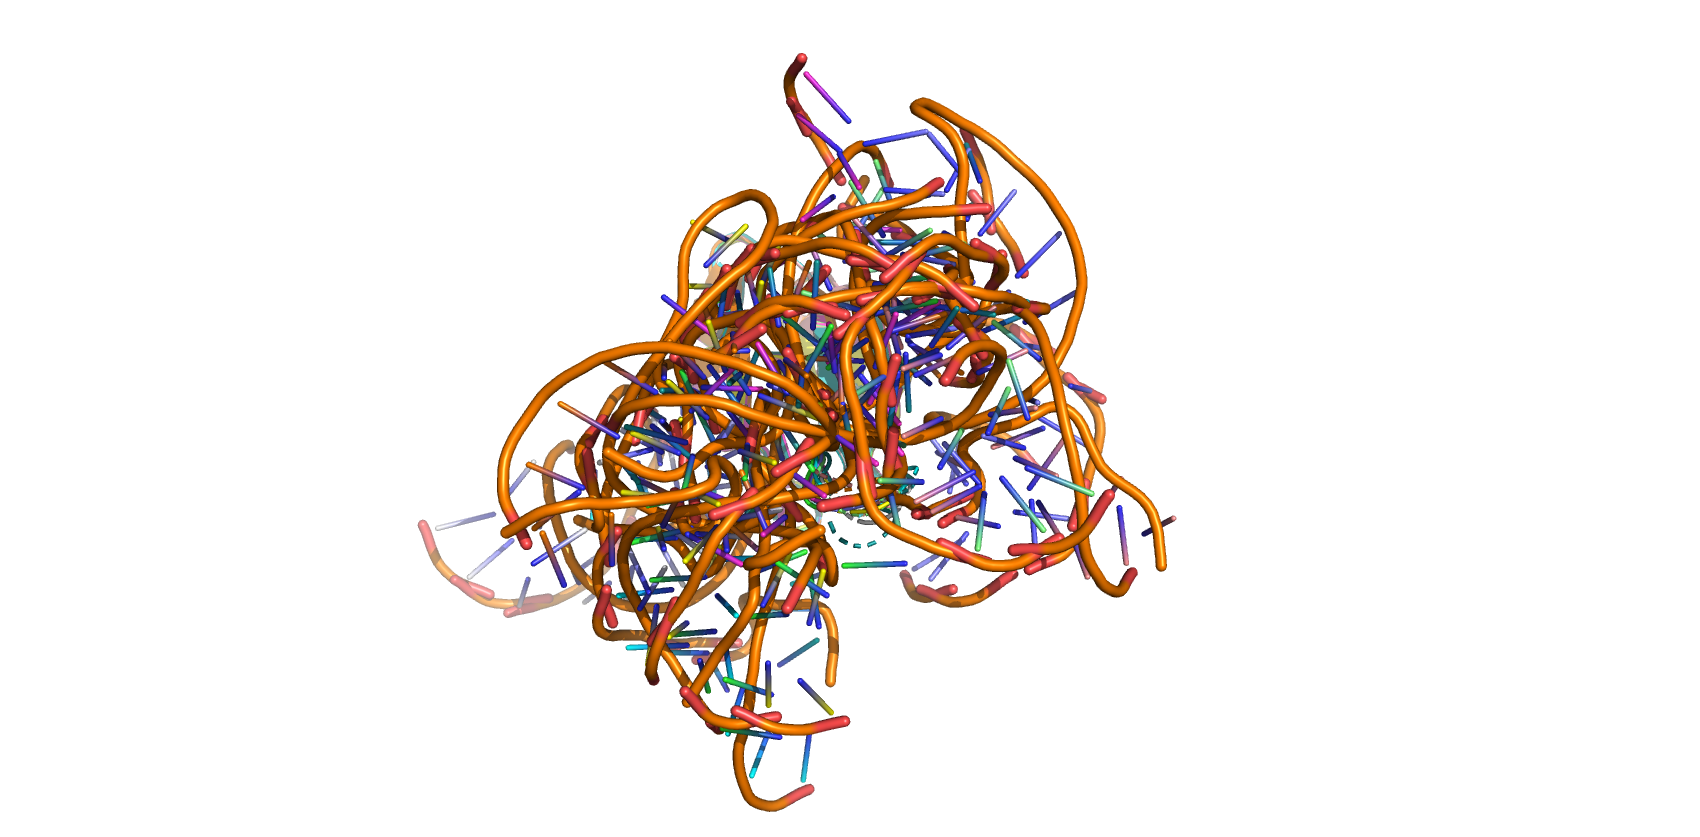
\includegraphics[trim={6.5cm 0 6.5cm 0},clip,width=\linewidth]{assets/RMM1_mut1_ALL.png}
    \endminipage\hfill
    \minipage{0.32\textwidth}
        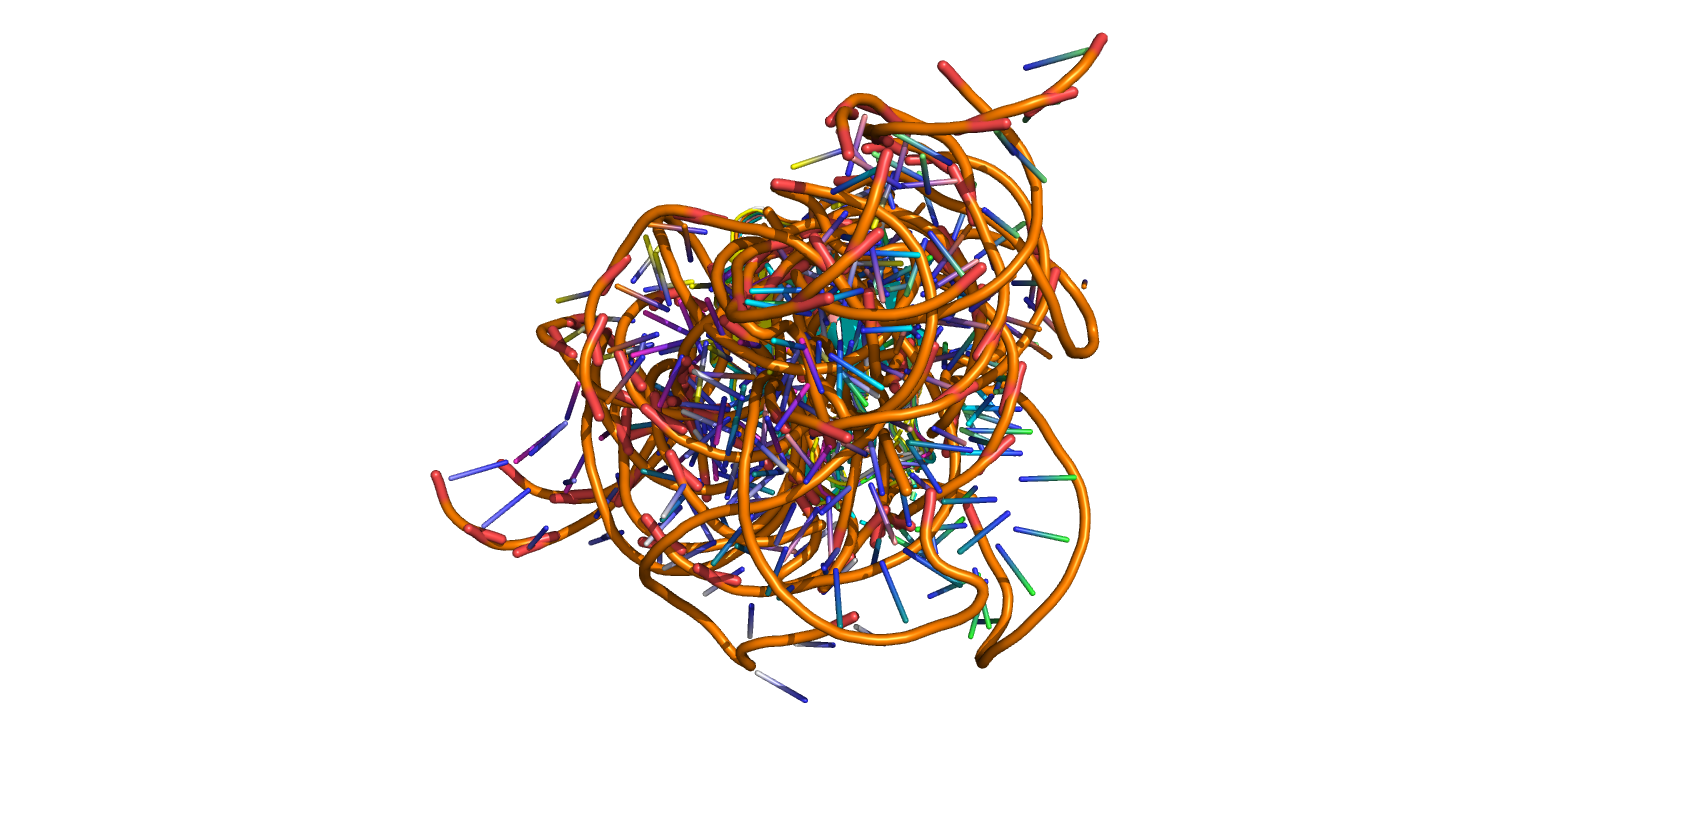
\includegraphics[trim={6.5cm 0 5.5cm 0},clip,width=\linewidth]{assets/RMM1_mut2_ALL.png}
    \endminipage\hfill
    \minipage{0.32\textwidth}
        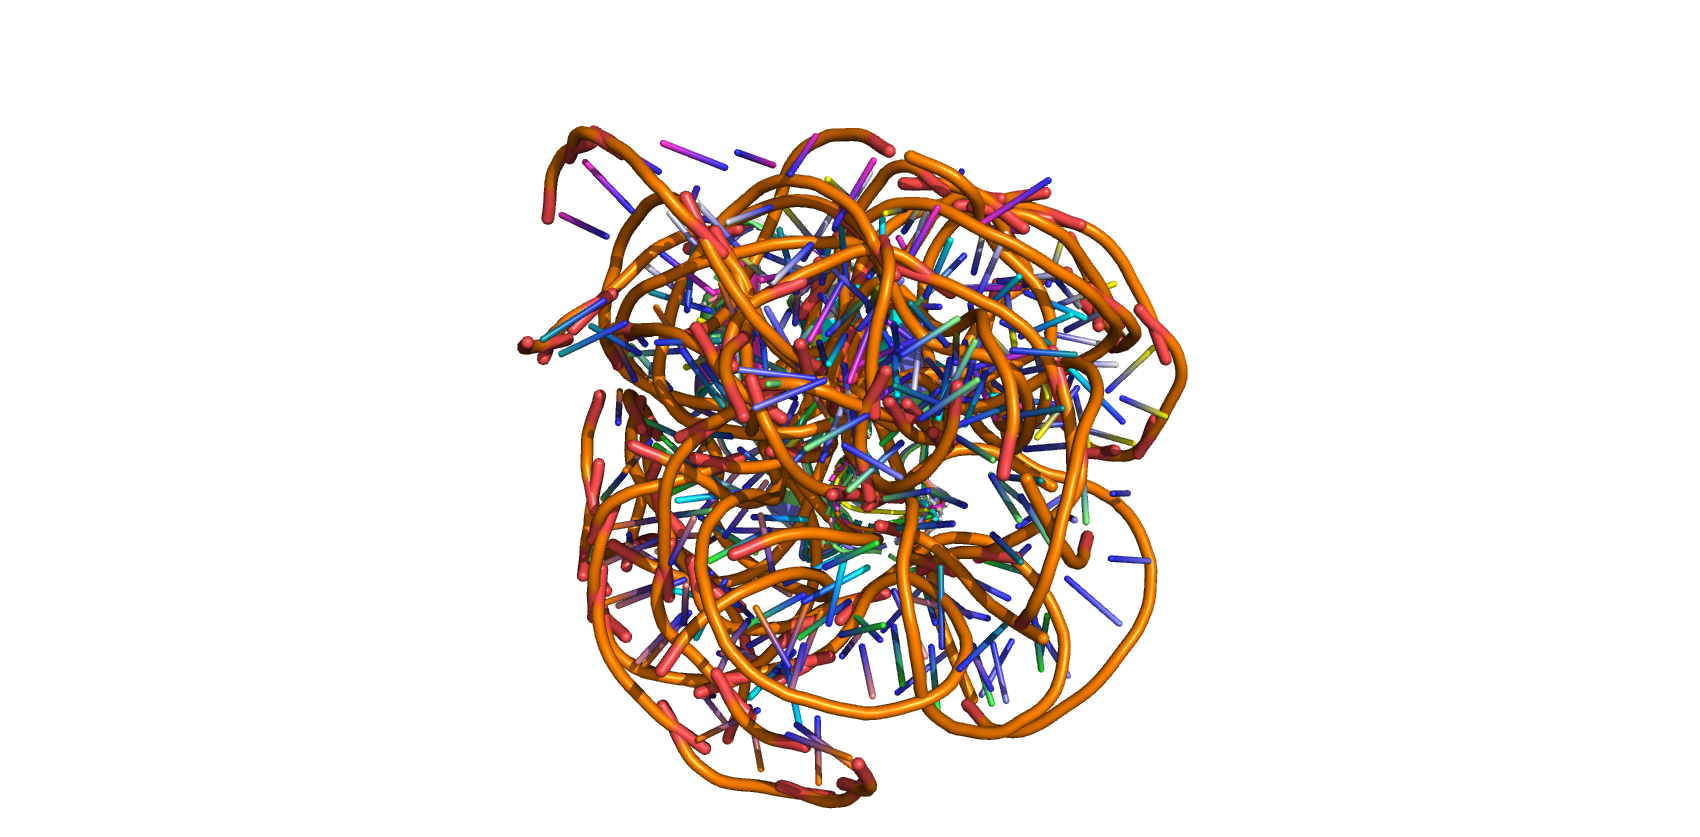
\includegraphics[trim={6.5cm 0 7cm 0},clip,width=\linewidth]{assets/RMM1_mut3_ALL.png}
    \endminipage\\
    \minipage{0.48\textwidth}
        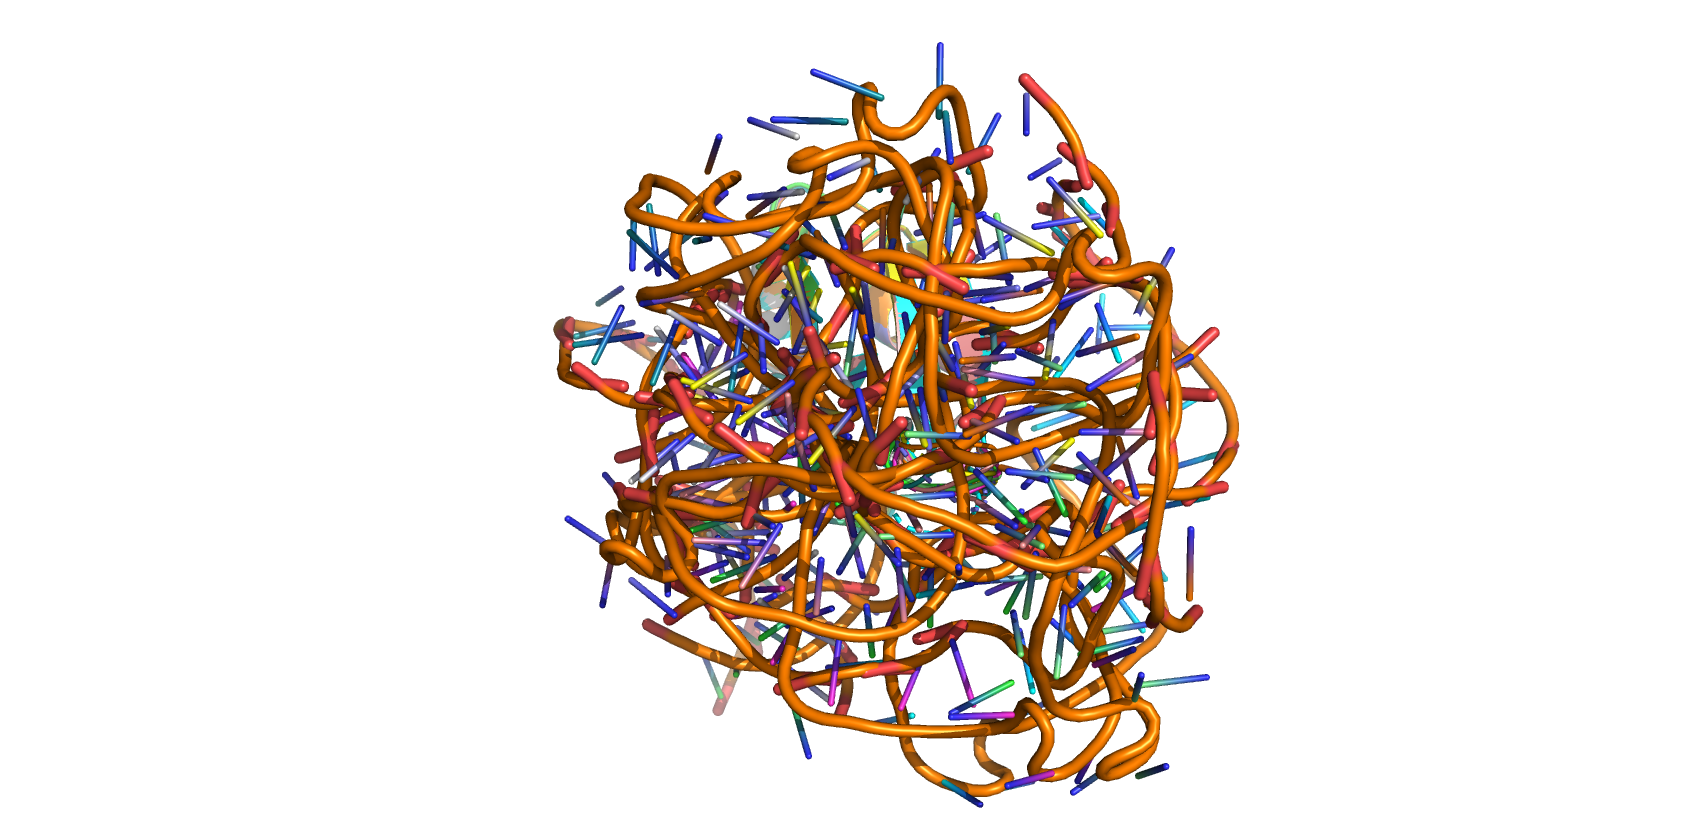
\includegraphics[trim={6.5cm 0 6.5cm 0},clip,width=\linewidth]{assets/RMM1_mut4_ALL.png}
    \endminipage\hfill
    \minipage{0.48\textwidth}
        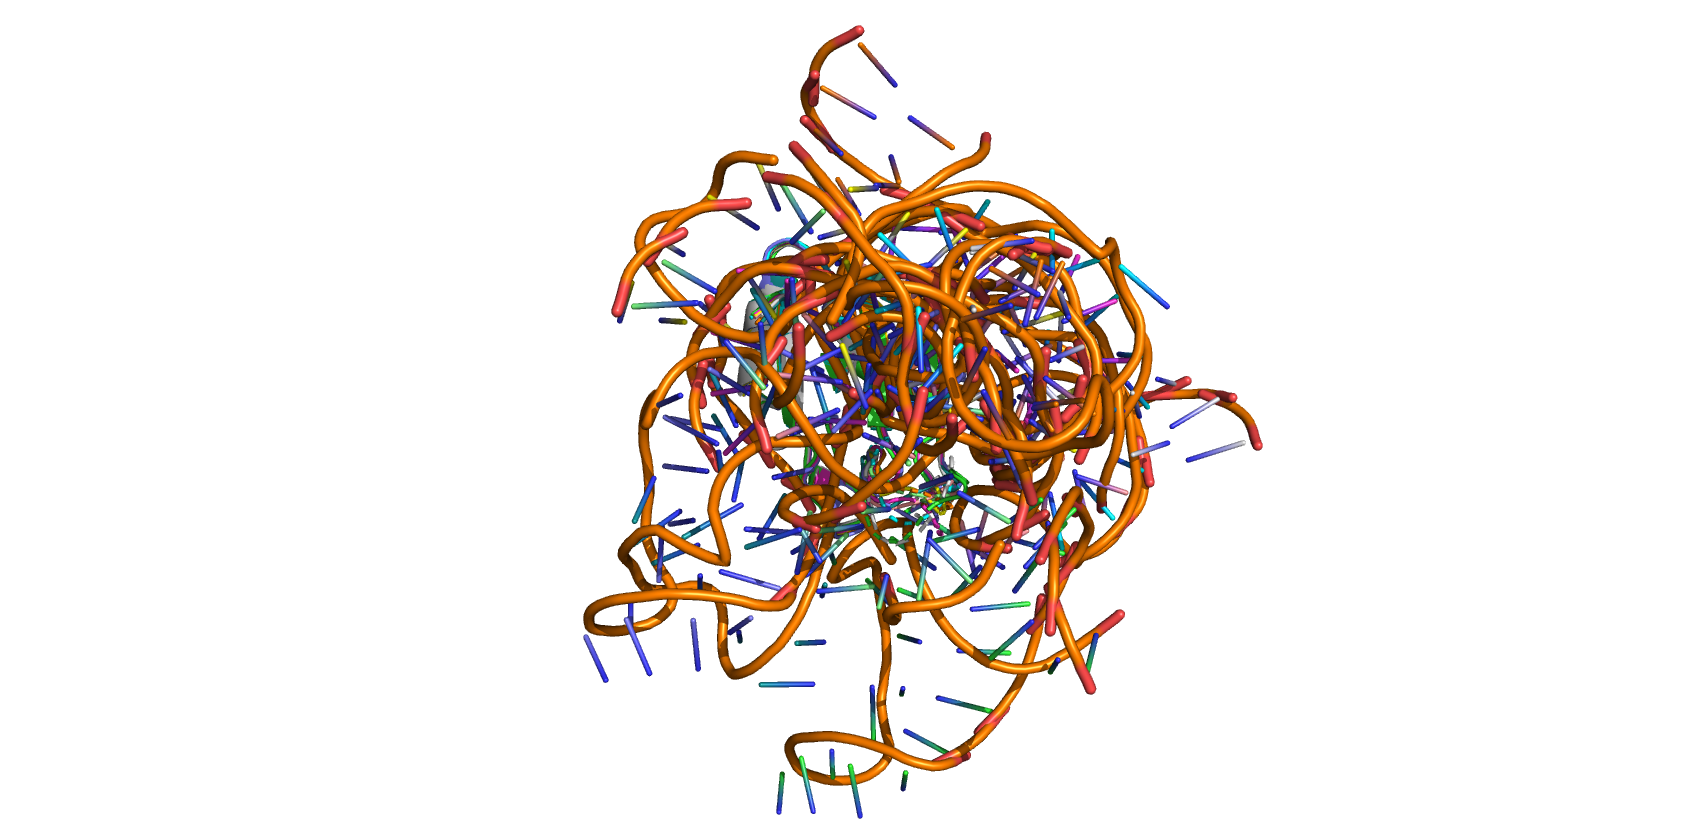
\includegraphics[trim={6.5cm 0 5.5cm 0},clip,width=\linewidth]{assets/RMM1_mut5_ALL.png}
    \endminipage
    \caption[Top 10 scoring models for RRM1-mutant RNA-motif complexes.]{Top 10 scoring models for RRM1-mutant RNA-motif complexes. From left to right and top to bottom: models for RRM1-mutant 1, RRM1-mutant 2, RRM1-mutant 3, RRM1-mutant 3 and RRM1-mutant 5. Visualized through \href{https://pymol.org/2/}{\texttt{Pymol}}.}
    \label{fig:RRMmuts}
\end{figure}

The resulting models do not reach consensus for any mutant and are unsatisfactory. This phenomenon contrasts with the models obtained for the original RNA motif, which are quite similar among them. Dolcemascolo and colleagues \cite{dolcemascolo_2022} designed these mutants in such a way that interaction between MSI-1 and the RNA was just slightly altered, observing in general a slight loss of affinity. An interaction similar to that of the original RNA motif was expected, which was also backed by the similarity of secondary structures among the original RNA motif and the mutants (especially for mutants 1, 2 and 3. See \textbf{Figure \ref{fig:RNAs}}).\\

It is surprising to observe that the supposed interaction is altered in such a drastic way by only point mutations. Thus, either MSI-1 is extremely sensitive with respect to the interacting RNA sequence or \textit{ab initio} docking is not sufficient to obtain good protein-RNA docking models.

\subsection{MSI-1's RRM1-lipid docking models}

The protein-lipid docking experiments were carried out with \texttt{AutoDock Vina}, and contrary to the previous docking simulations shown within this work, were not \textit{ab initio} as the spatial region where the fatty acid is supposed to interact was given as a constraint. Given the polarity of MSI1's RRM1's surface (see \textbf{Figure \ref{fig:RRM1polarity}}), especially within the fatty acid-binding pocket, it is expected for the fatty acid to expose their carboxylic head outwards (towards the liquid medium) while hiding their nonpolar tail within the binding pocket.

\begin{figure}[htbp!]
    \centering
    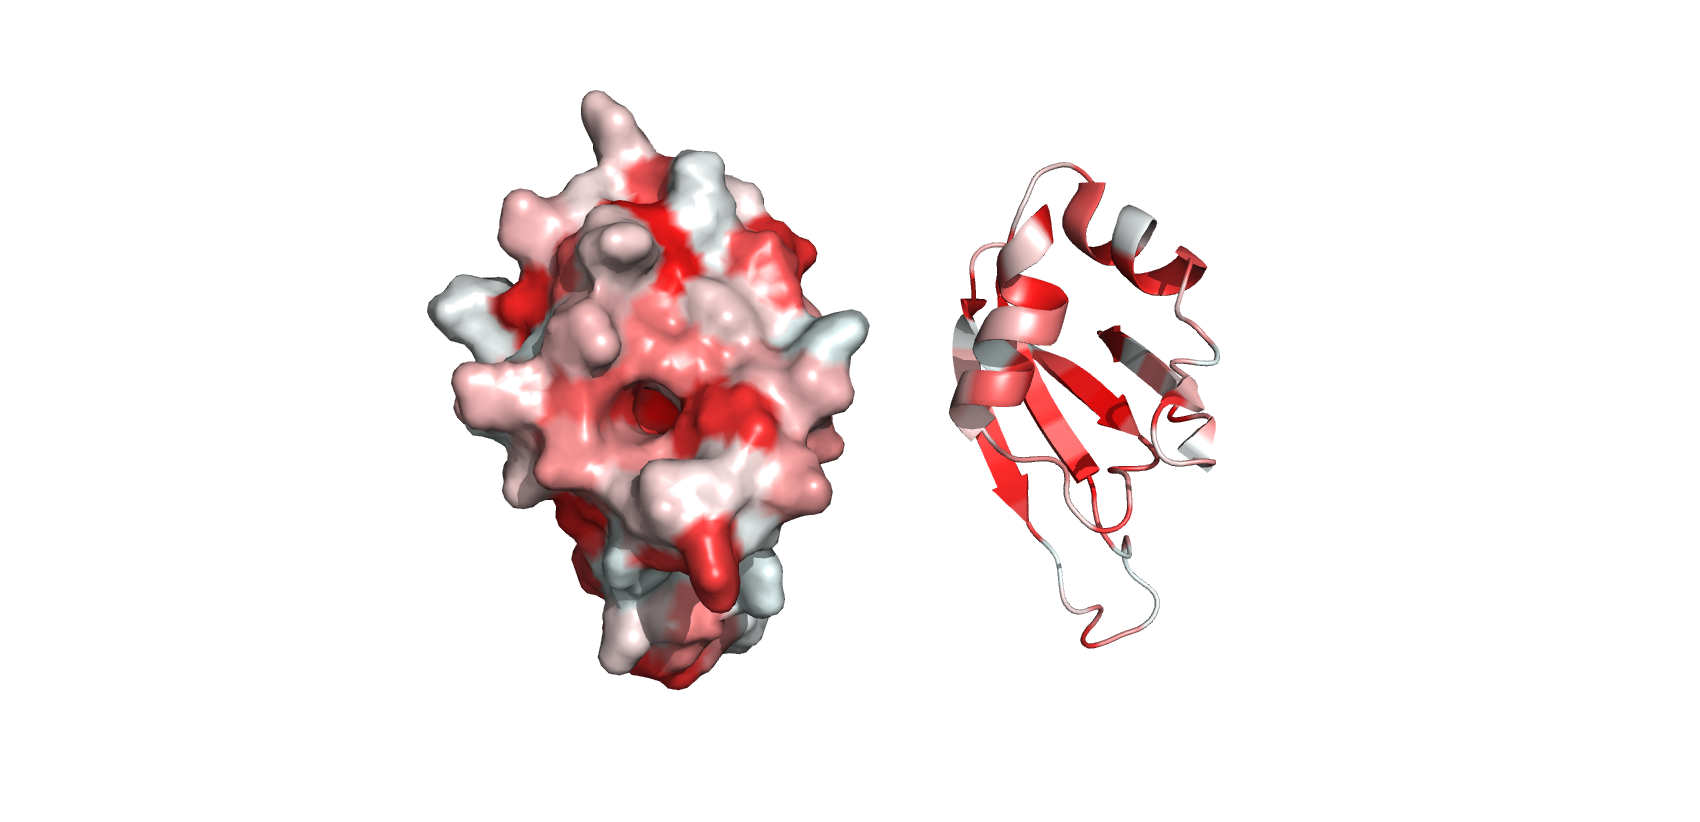
\includegraphics[width=\linewidth]{assets/RRM1_colored_polarity.png}
    \caption[MSI1's RRM1 colored by aminoacid polarity.]{MSI1's RRM1 colored by aminoacid polarity. The leftmost representation is surface representation while the rightmost is the cartoon of the secondary structure. The intensity of red indicates the degree of non-polarity.}
    \label{fig:RRM1polarity}
\end{figure}

With this criterion in mind, it is easy to select the models that are less likely to happen in nature: the models in which the carboxylic group is hidden within the binding pocket.\\

The best structures (chosen by score and following the previous criterion) are shown in \textbf{Figure \ref{fig:fattyAcidModels}}:

\begin{figure}[htbp!]
    \minipage{0.32\textwidth}
        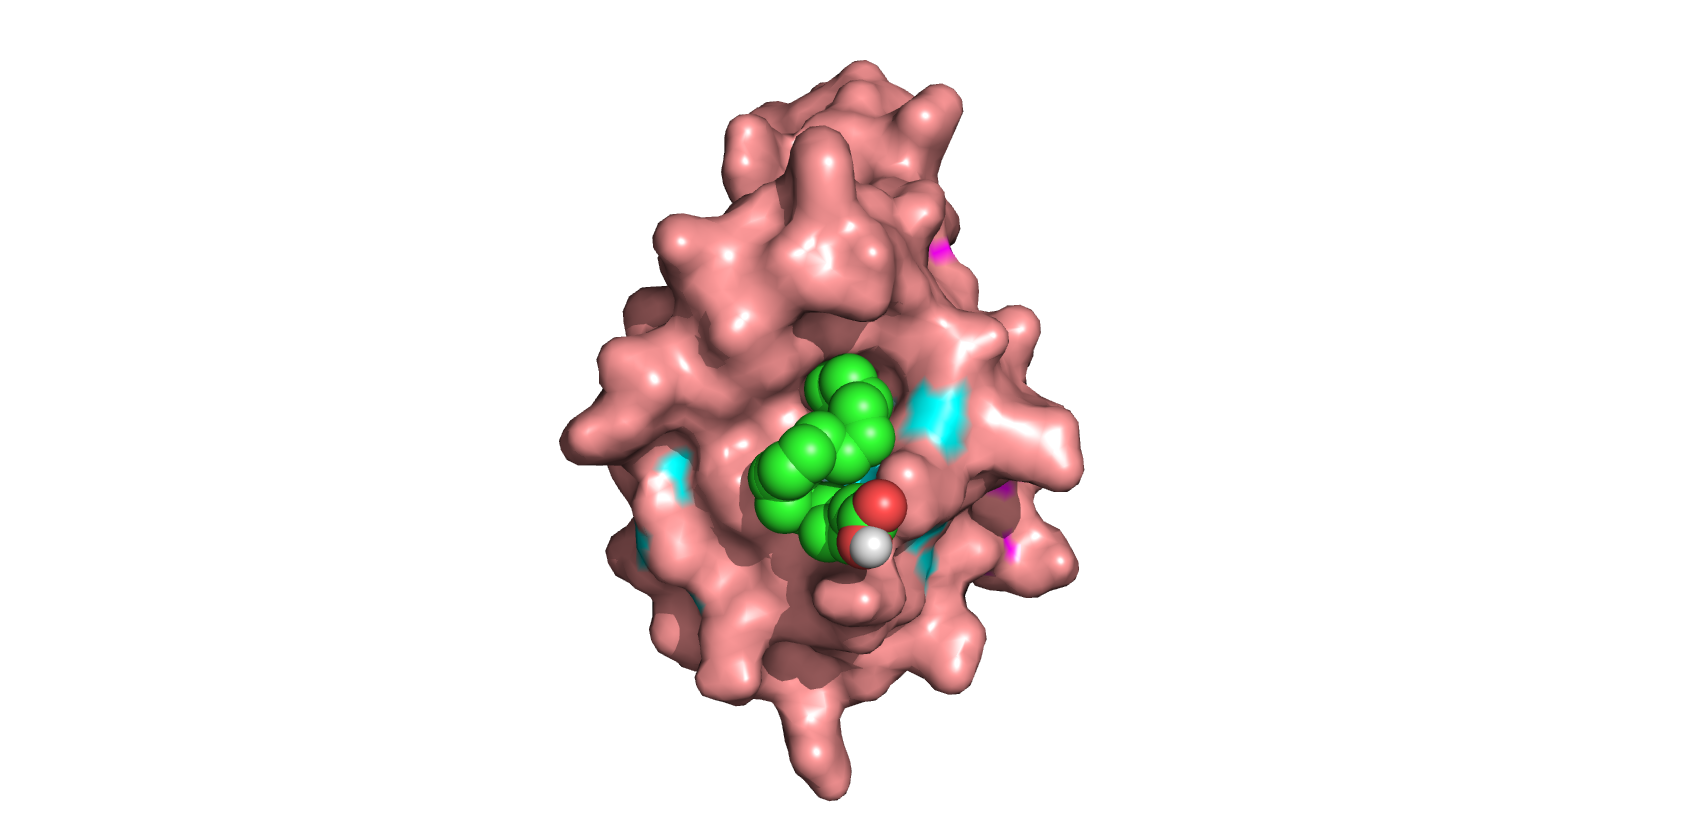
\includegraphics[trim={6.5cm 0 6.5cm 0},clip,width=\linewidth]{assets/RRM1_oleic_solo.png}
    \endminipage\hfill
    \minipage{0.32\textwidth}
        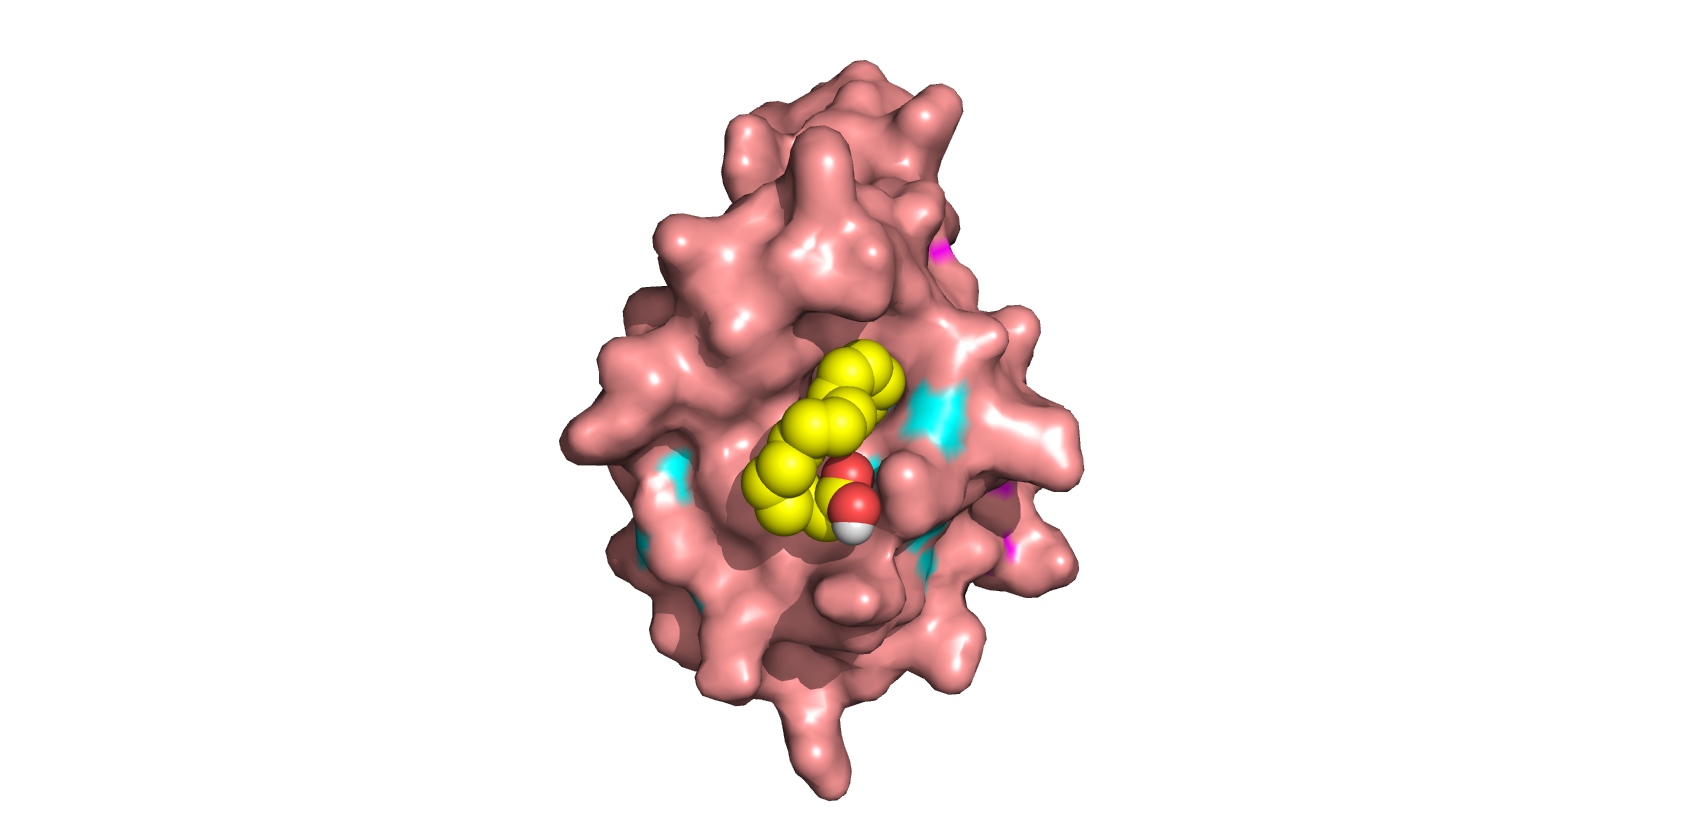
\includegraphics[trim={6.5cm 0 5.5cm 0},clip,width=\linewidth]{assets/RRM1_linoleic_solo.png}
    \endminipage\hfill
    \minipage{0.32\textwidth}
        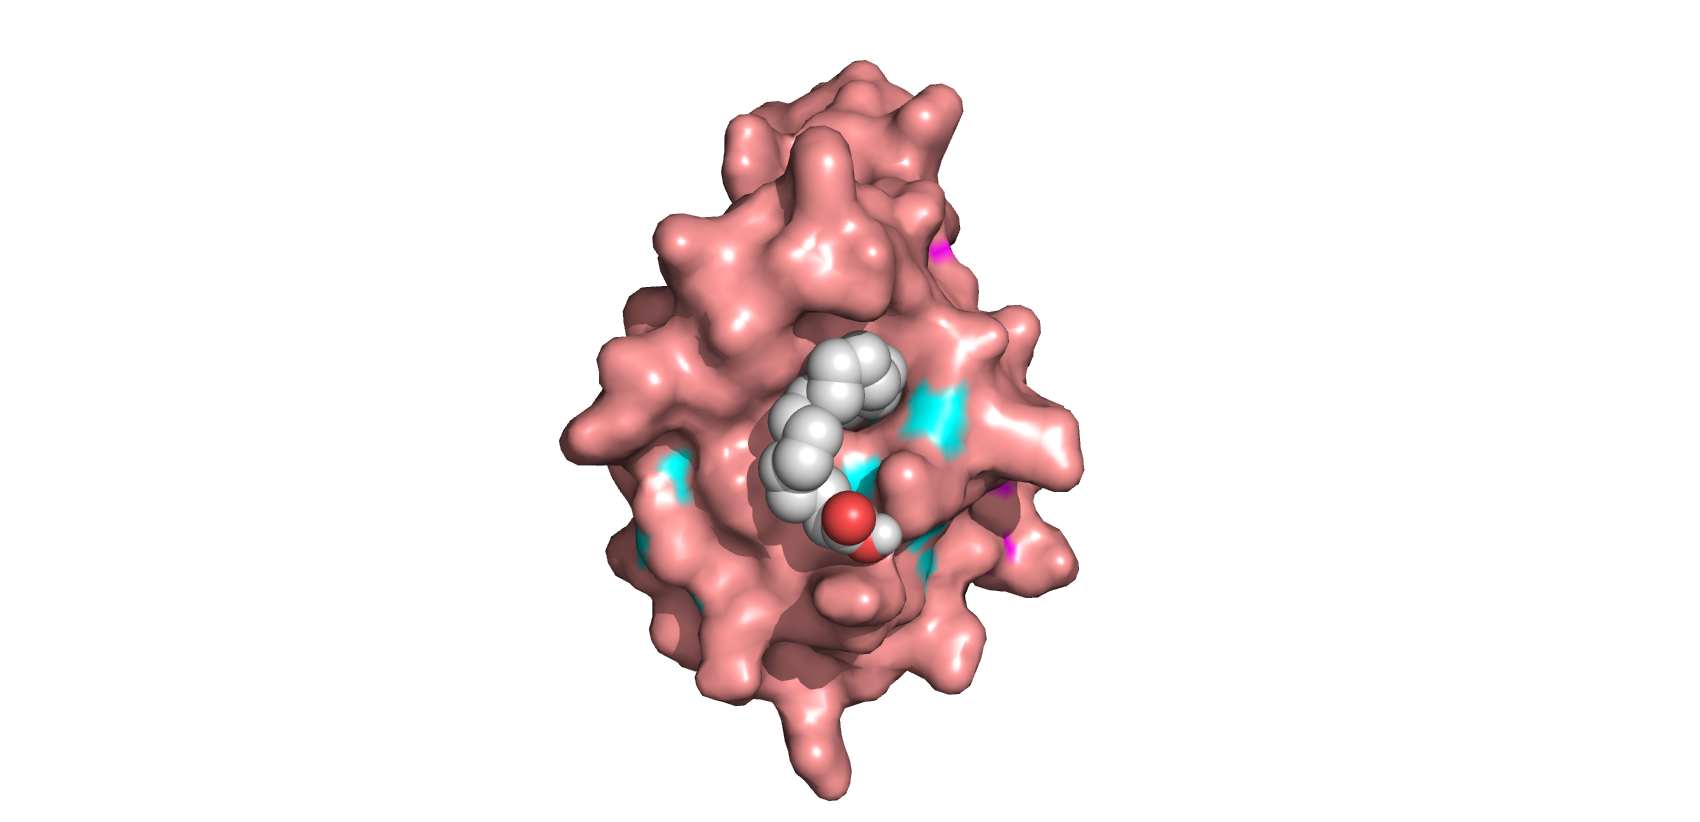
\includegraphics[trim={6.5cm 0 7cm 0},clip,width=\linewidth]{assets/RRM1_stearic_solo.png}
    \endminipage\\
    \minipage{0.48\textwidth}
        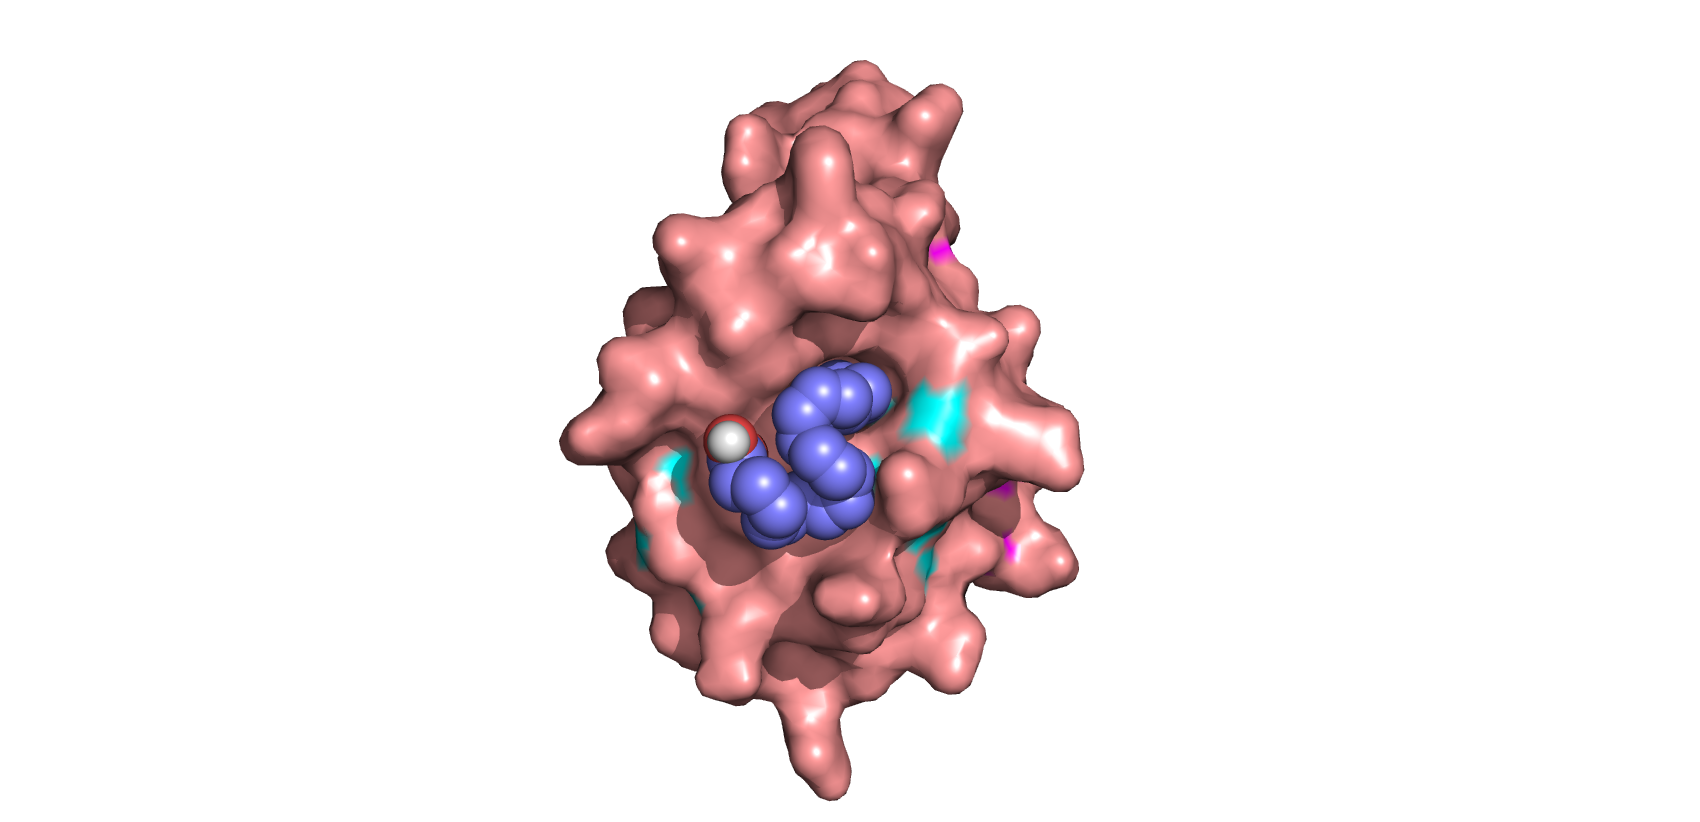
\includegraphics[trim={6.5cm 0 6.5cm 0},clip,width=\linewidth]{assets/RRM1_arachidonic_solo.png}
    \endminipage\hfill
    \minipage{0.48\textwidth}
        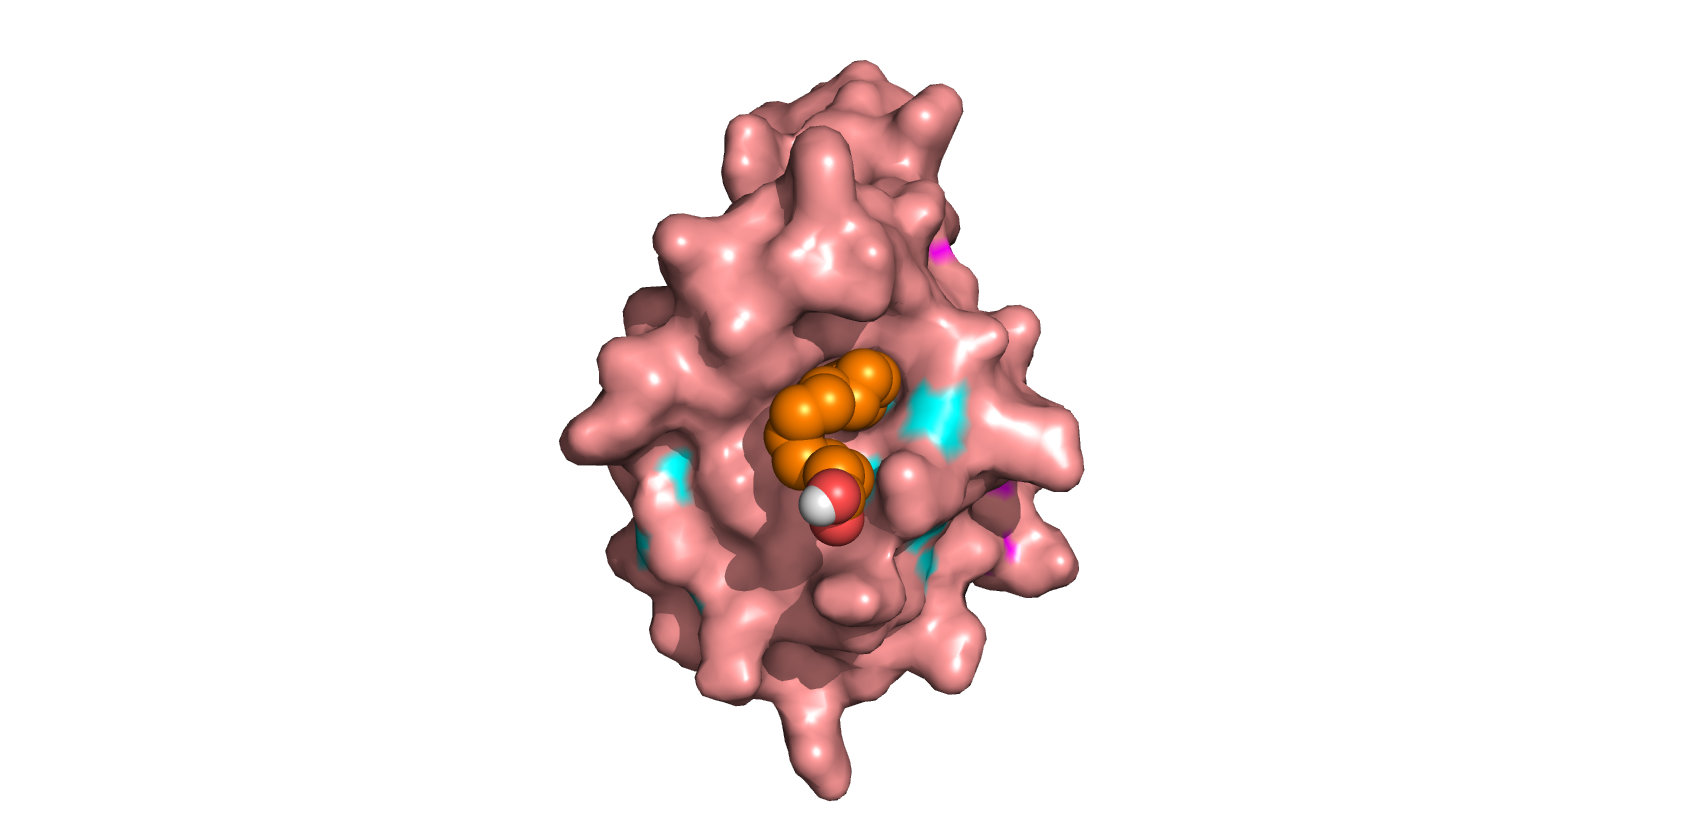
\includegraphics[trim={6.5cm 0 5.5cm 0},clip,width=\linewidth]{assets/RRM1_palmitic_solo.png}
    \endminipage
    \caption[Top models for RRM1-fatty acid docking simulations.]{Top models for RRM1-fatty acid docking simulations. From left to right and top to bottom: models for RRM1-oleic acid (green), RRM1-linoleic acid (yellow), RRM1-stearic acid (white), RRM1-arachidonic acid (purple) and RRM1-palmitic acid (orange). Visualized through \href{https://pymol.org/2/}{\texttt{Pymol}}.}
    \label{fig:fattyAcidModels}
\end{figure}

The models selected are satisfactory as they hide most of the hydrophobic chain within the pocket. In addition, the polar carboxylic group interacts with the surface of the protein as expected. Apparently, the less flexible the fatty acid's chain (see for example arachidonic acid), the more constrained the interaction is and the harder it is for it actually to happen.\\

In contrast, short and flexible fatty acids (see for example oleic acid), the easier the interaction is and thus, it is easier for it to happen. These results agree with Clingman and colleagues' findings \cite{clingman_2014}.

\subsection{Lipid-protein-RNA complex visualization}

The construction and visualization of the lipid-protein-RNA complexes was done by loading the protein-RNA docking models and the protein lipid docking models, and then manually superposing them so that all structures had cohesion within \href{https://pymol.org/2/}{\texttt{Pymol}}.\\

Since the protein-mutant RNA motifs docking models did not reach consensus, it only is reliable to build the lipid-protein-RNA complex with the original RNA. The oleic acid-RRM1-original RNA motif complex is shown in \textbf{Figure \ref{fig:oleicOrigComplex}}:

\begin{figure}[htbp!]
    \minipage{0.48\textwidth}
        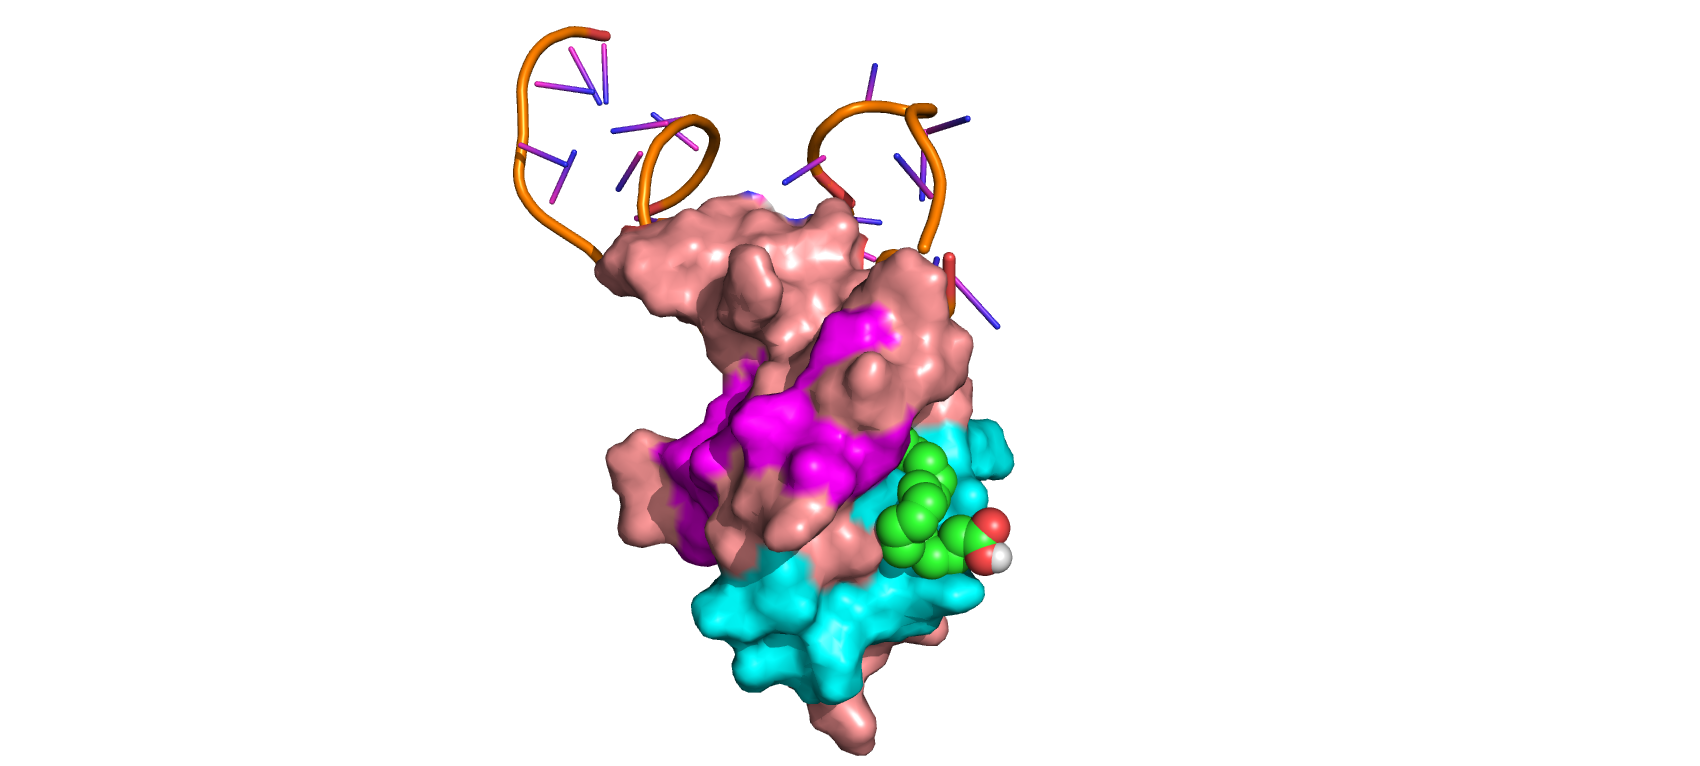
\includegraphics[trim={6.5cm 0 5.5cm 0},clip,width=\linewidth]{assets/RRM1_orig_oleic1.png}
    \endminipage\hfill
    \minipage{0.48\textwidth}
        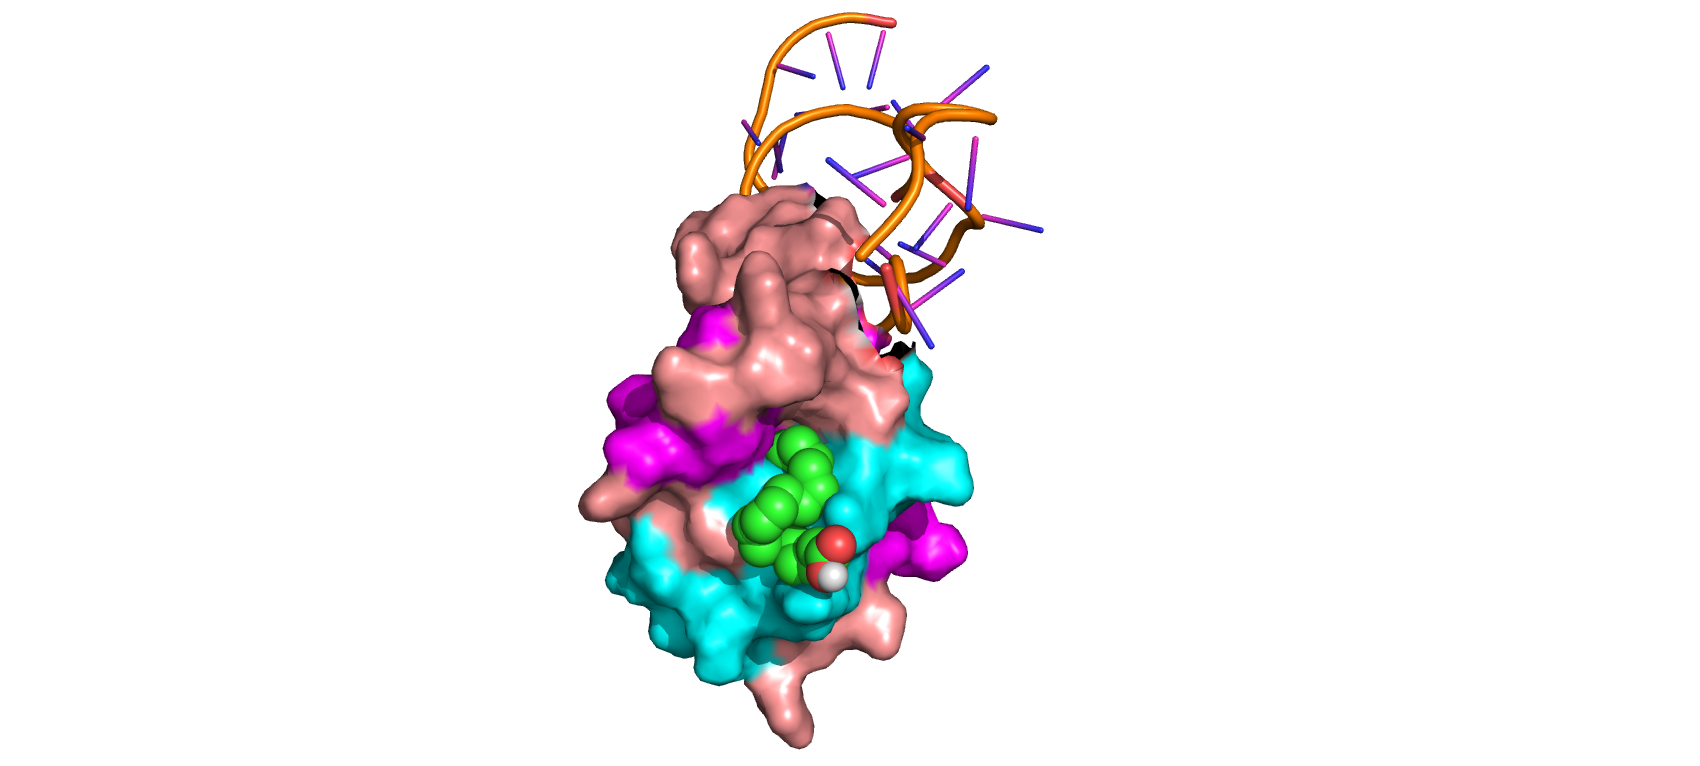
\includegraphics[trim={6.5cm 0 7cm 0},clip,width=\linewidth]{assets/RRM1_orig_oleic2.png}
    \endminipage
    \caption[Oleic acid-RRM1-original RNA motif complex.]{Oleic acid-RRM1-original RNA motif complex. The leftmost structure is a side view while the rightmost structure is a front view. Visualized through \href{https://pymol.org/2/}{\texttt{Pymol}}.}
    \label{fig:oleicOrigComplex}
\end{figure}

As expected, the locations at which the RNA motif and the oleic acid attach are clearly different: the RNA motif attaches around the \texttt{DPLTKRS} loop while the oleic acid enters a pocket located on the opposite face of the protein. The distance among these binding sites and the size of the molecules discards the RNA-binding inhibition due to steric impediment and confirms that inhibition is in fact an allosteric behavior.\\

This allosterism must stem from a conformational change deep within the protein due to the non-polar nature of the oleic acid-RRM1 interaction. The conformational change must then be transmitted to the opposite face of the protein, altering the RNA binding site and thus causing a chance for release.\\

The remaining complexes, which originate from employing the other fatty acids, are constructed as well. These are shown in \textbf{Figure \ref{fig:complexesFinal}}:\pagebreak

\begin{figure}[htbp!]
    \minipage{0.48\textwidth}
        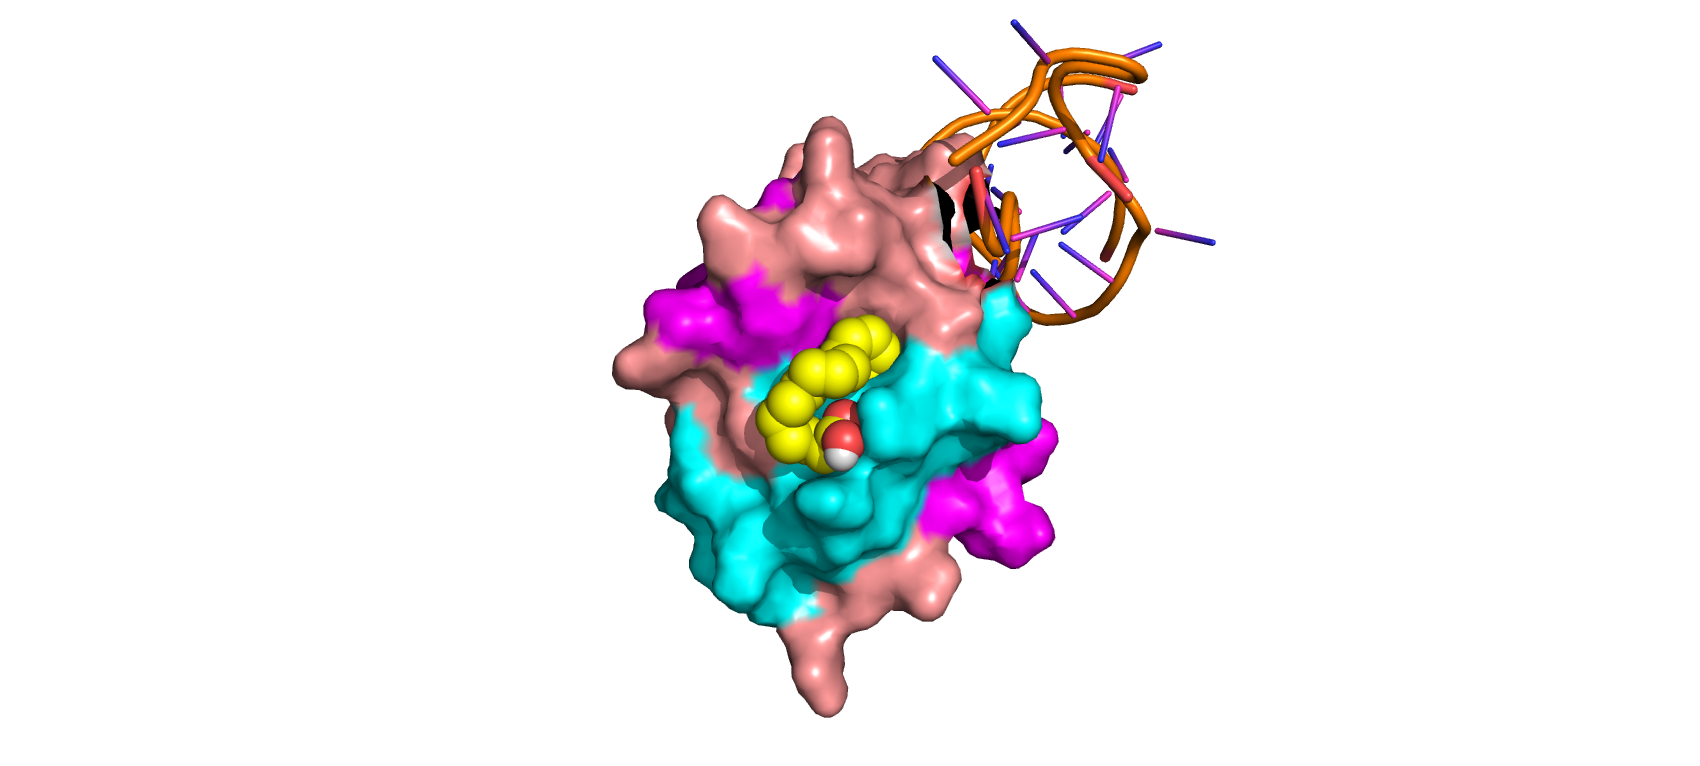
\includegraphics[trim={6.5cm 0 5.5cm 0},clip,width=\linewidth]{assets/RRM1_orig_linoleic.png}
    \endminipage\hfill
    \minipage{0.48\textwidth}
        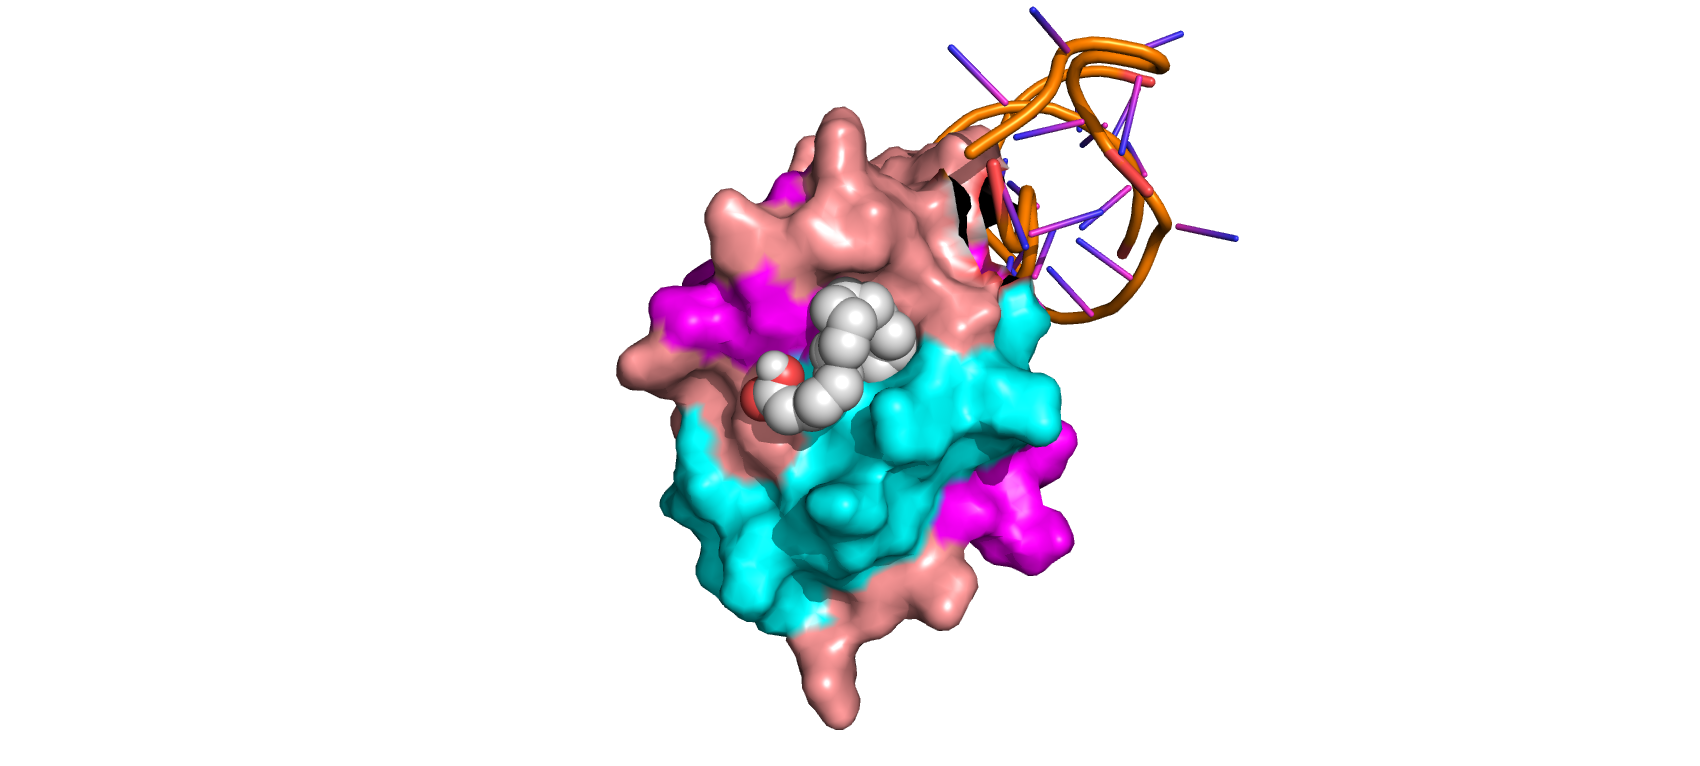
\includegraphics[trim={6.5cm 0 7cm 0},clip,width=\linewidth]{assets/RRM1_orig_stearic.png}
    \endminipage\\
    \minipage{0.48\textwidth}
        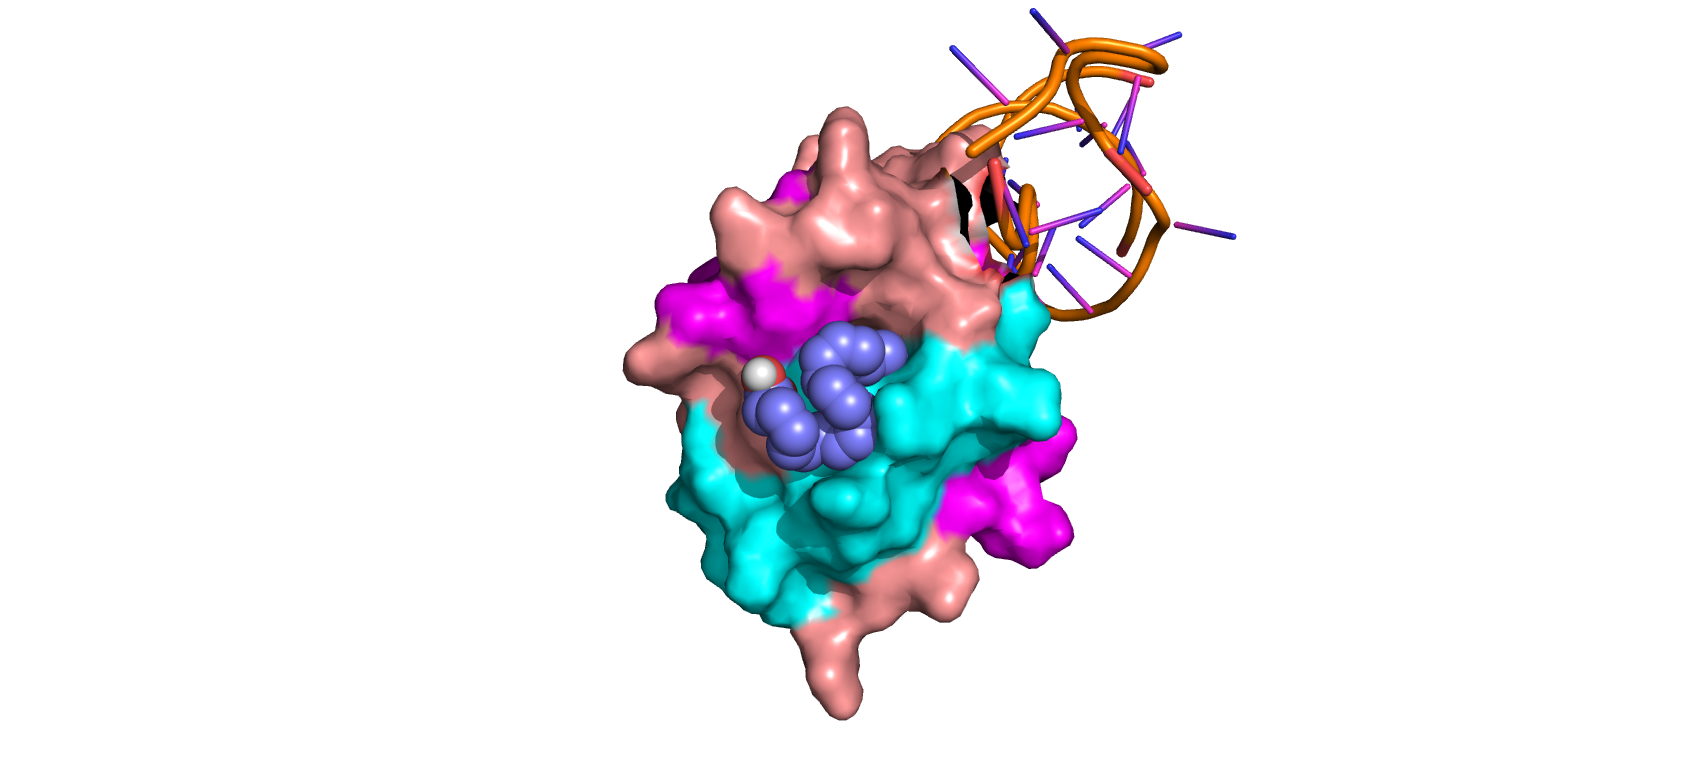
\includegraphics[trim={6.5cm 0 6.5cm 0},clip,width=\linewidth]{assets/RRM1_orig_arachidonic.png}
    \endminipage\hfill
    \minipage{0.48\textwidth}
        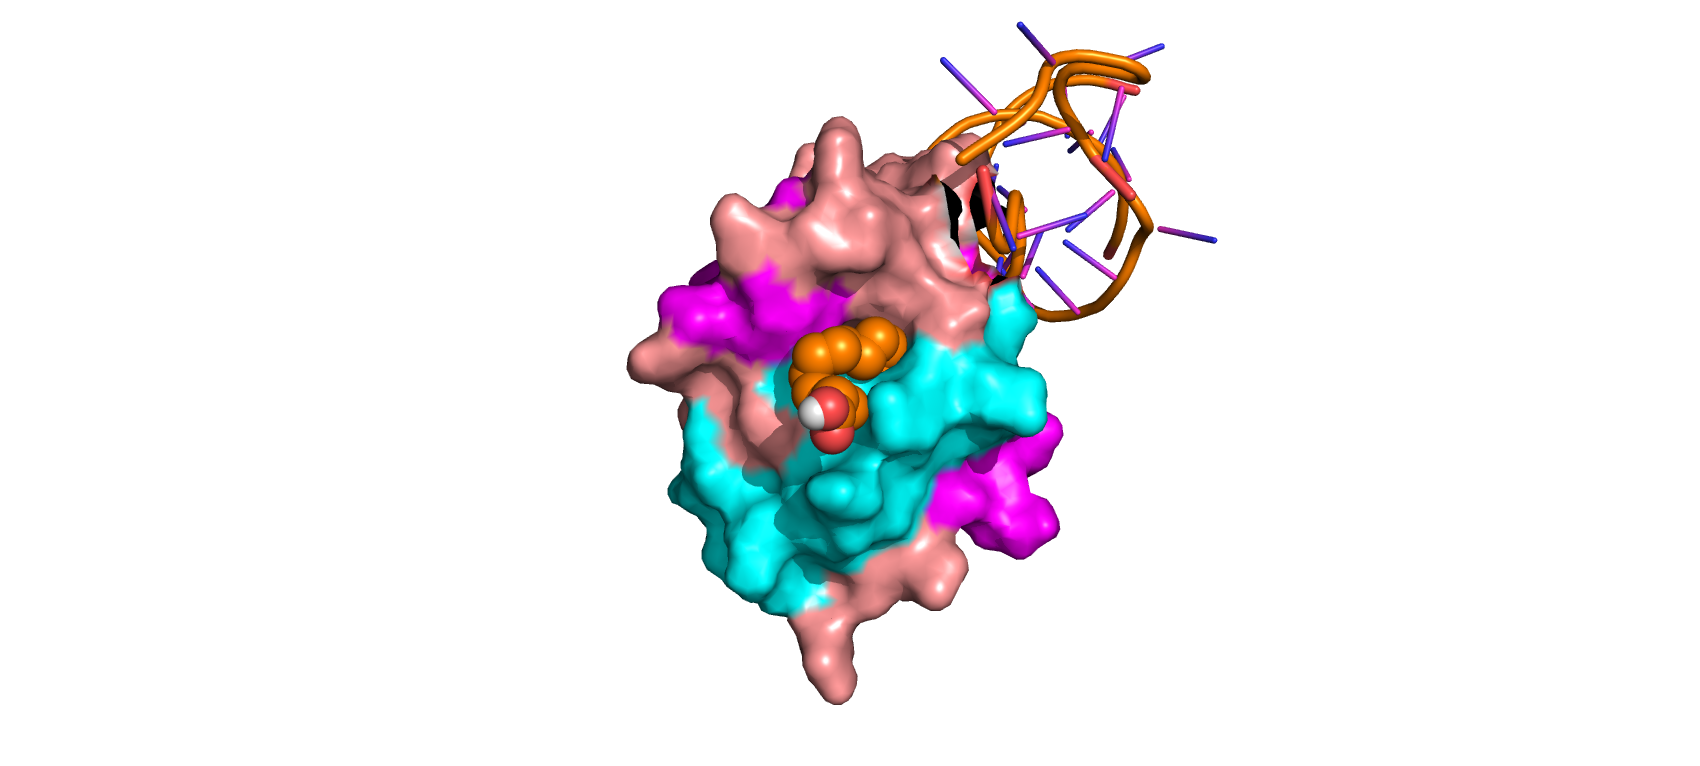
\includegraphics[trim={6.5cm 0 5.5cm 0},clip,width=\linewidth]{assets/RRM1_orig_palmitic.png}
    \endminipage
    \caption[Top models for RRM1-fatty acid complexes.]{Top models for RRM1-fatty acid complexes. From left to right and top to bottom: models for RRM1-oleic acid (green), RRM1-linoleic acid (yellow), RRM1-stearic acid (white), RRM1-arachidonic acid (purple) and RRM1-palmitic acid (orange). Visualized through \href{https://pymol.org/2/}{\texttt{Pymol}}.}
    \label{fig:complexesFinal}
\end{figure}

For the remaining fatty acids, the same reasoning holds: interactions occur in different faces of the protein, and the distance among sites, plus the small size of the ligands, discard steric impediments.\\